\chapter{Analyse en composantes principales}

\myminitoc

\sect{Introduction - Maximisation de la variance}

L'\textbf{analyse de composante principale (PCA)} est une réduction de la dimension. Elle projette un ensemble de points vivant dans un espace de dimension {\boldmath $d$} sur un sous-espace de dimension {\boldmath $M$}~$< d$. Si $M = 2$ alors on peut visualiser les données. L'analyse génère de nouvelles features qui sont décorrélés et qui un sens qui permet de bien discriminer les données.

\begin{center}
	\begin{tikzpicture}[thick]
		\draw[purple, very thick] (0, -0.846) -- (8, 3.804);
		\draw[greenTikz] (0.491, 0.039) -- (0.751, -0.409);
		\draw[fill=red] (0.491, 0.039) circle (0.15);
		\draw[fill=greenTikz] (0.751, -0.409) circle (0.15);
		\draw[greenTikz] (3.370, 0.587) -- (3.141, 0.980);
		\draw[fill=red] (3.370, 0.587) circle (0.15);
		\draw[fill=greenTikz] (3.141, 0.980) circle (0.15);
		\draw[greenTikz] (1.769, -0.248) -- (1.582, 0.073);
		\draw[fill=red] (1.769, -0.248) circle (0.15);
		\draw[fill=greenTikz] (1.582, 0.073) circle (0.15);
		\draw[greenTikz] (5.370, 3.037) -- (5.701, 2.468);
		\draw[fill=red] (5.370, 3.037) circle (0.15);
		\draw[fill=greenTikz] (5.701, 2.468) circle (0.15);
		\draw[greenTikz] (6.241, 2.376) -- (6.064, 2.679);
		\draw[fill=red] (6.241, 2.376) circle (0.15);
		\draw[fill=greenTikz] (6.064, 2.679) circle (0.15);
	\end{tikzpicture} \\
	Ici $d=2$ et $M=1$.
	\vspace{1mm}
\end{center}

Supposons que notre ensemble d'entraînement a une moyenne nulle, (cela peut être obtenu en remplaçant les $x_i$ par $x_i - \bar{x}$). PCA cherche une transformation linéaire $U$ qui à $x_i$ associera le nouveau point :
$$ t_i = U^\trans x_i $$
Où $U = (u_1, ..., u_M)$ est une matrice de dimension $d \times M$. Les vecteurs $u_j$ représentent une base de notre sous espace de $R^d$. De plus on souhaite que la base soit orthonormale. On obtient donc la contrainte suivante :
$$ U^\trans U = I_M $$
On peut aussi définir la reconstruction d'un point du nouveau sous-espace par $\hat{x}_i = U t_i$. Dans ce cas on veut minimiser l'erreur quadratique moyenne $J(U)$ entre $x$ et $\hat{x}$ tout en essayant de garder $M$ aussi petit que possible.
$$ \begin{array}{lll}
\displaystyle \min_U J(U)
& = & \displaystyle \min_U~\dfrac{1}{n} \sum_i (x_i - \hat{x}_i)² \\
& = & \displaystyle \min_U~\dfrac{1}{n} \sum_i (x_i - UU^\trans x_i)^\trans (x_i - UU^\trans x_i) \\
& = & \displaystyle \min_U~\dfrac{1}{n} \sum_i (x_i^\trans x_i - 2 xi^\trans UU^\trans x_i + x_i^\trans U U^\trans U U^\trans x_i)
\end{array} $$
On utilise alors la contrainte $U^\trans U = I_M$ :
$$ \begin{array}{lll}
\displaystyle \min_U J(U)
& = & \displaystyle \min_U~\dfrac{1}{n} \sum_i (x_i^\trans x_i - xi^\trans UU^\trans x_i) \\
& = & \displaystyle \min_U~\dfrac{1}{n} \sum_i (x_i^\trans x_i - t_i^\trans t_i) \\
& = & \displaystyle \min_U~tr \left( \dfrac{1}{n} \sum_i x_i x_i^\trans - t_i t_i^\trans \right) \\
& = & \displaystyle \min_U~tr \left( \dfrac{1}{n} \sum_i x_i x_i^\trans - U^\trans x_i x_i^\trans U \right) \\
& = & \displaystyle \min_U~tr \left( \dfrac{1}{n} \sum_i x_i x_i^\trans \right) - tr \left( \dfrac{1}{n} \sum_i U^\trans x_i x_i^\trans U \right) \\
& = & \displaystyle \min_U~tr \left( \dfrac{1}{n} \sum_i x_i x_i^\trans \right) - tr \left( U^\trans \left( \dfrac{1}{n} \sum_i x_i x_i^\trans \right) U \right) \\
& = & \displaystyle \min_U~tr \left( \Sigma \right) - tr \left( U^\trans \Sigma U \right)
\end{array} $$
Où {\boldmath $\Sigma$} est la \textbf{matrice de covariance} des données d'origine et $U^\trans \Sigma U$ est la matrice de covariance dans le nouvelle espace. \\
Comme $tr(\Sigma)$ ne dépend pas de $U$ minimiser $J(U)$ revient à maximiser $tr(U^\trans \Sigma U)$. On obtient donc le problème suivant :
\begin{center}
	\fbox{
	\parbox{7cm}{
	$$ \max_{u_1, ..., u_M} \sum_j u_j^\trans \Sigma u_j $$
	\vspace{-4mm}
	$$ \text{s.t.} \quad \forall j, k \in \{ 1, ..., M \}, \, u_j^\trans u_k = \delta_{j, k} $$
	\vspace{-4mm}
	}
	}
\end{center}

\sect{Solution de forme fermée}

La matrice de covariance $\Sigma$ est symétrique donc en utilisant le théorème spectrale on obtient l'existence d'une matrice diagonale $D = diag(\lambda_1, ..., \lambda_d)$ et l'existence d'une matrice orthogonale $V$ tel que $\Sigma = V D V^\trans$. On ordonne les valeurs propres de $\Sigma$ de telle sorte que $\lambda_1 \geqslant ... \geqslant \lambda_d$. \\
On cherche donc à maximiser la valeur suivante :
$$ \begin{array}{lll}
\displaystyle \sum_j u_j^\trans \Sigma u_j
& = & \displaystyle \sum_j u_j^\trans V D V^\trans u_j \\
& = & \displaystyle \sum_j \left( V^\trans u_j \right)^\trans D \left( V^\trans u_j \right) \\
& = & \displaystyle \sum_{i, j} \left( v_i^\trans u_j \right) \lambda_i \left( v_i^\trans u_j \right) \\
& = & \displaystyle \sum_{i, j} \lambda_i \left( v_i^\trans u_j \right)^2 \\
\end{array} $$
Comme les $(u_j)$ forment une famille orthonormale, on peut la compléter par des vecteurs $w_{M+1}, ..., w_d$ pour former une base orthonormale. Ainsi la matrice formé des colonnes $W = (u_1, ..., u_M, w_{M+1}, ..., w_d)$ est une matrice orthogonale. Comme $V$ est aussi orthogonale, le produit $V^\trans W$ est une matrice orthogonale. Puis, en utilisant le fait que les lignes d'une matrice orthogonale sont de norme 1, on obtient :
$$ \forall i, \quad \alpha_i = \sum_{j = 1}^M \left( v_i^\trans u_j \right)^2 = 1 - \sum_{j = M+1}^d \left( v_i^\trans w_j \right)^2 \leqslant 1 $$
De plus, les vecteurs $(v_i)$ formant une base orthonormé, on obtient $\sum_i \left( v_i^\trans u_j \right)^2 = u_j^\trans u_j = 1$. D'où :
$$ \sum_i \alpha_i = \sum_{i, j} \left( v_i^\trans u_j \right)^2 = M $$
Notre problème s'écrit alors :
$$ \max_\alpha \sum_i \lambda_i \alpha_i $$
\vspace{-2mm}
$$ \text{s.t.} \quad \left\{ \begin{array}{l}
\forall i, \, \alpha_i \leqslant 1 \\
\sum_i \alpha_i = M
\end{array} \right. $$
Une solution optimale est alors $\alpha_i = 1$ si $i \leqslant M$ et $\alpha_i = 0$ si $i > M$. Ces valeurs de $\alpha_i$ peuvent être obtenue avec $u_j = v_j$. \\
{\boldmath \textbf{Trouver} $U$ \textbf{revient alors à trouver les vecteurs propres correspondant aux plus grandes valeurs propres de} $\Sigma$}.

\paragraph{Qualité de la projection}
Pour ne pas perdre d'information on peut prendre $M$ le nombre de valeurs propres non nulles de $\Sigma$. La somme des valeurs propres correspond à la variance de données. Si on s'autorise une perte de variance, on peut alors définir le ratio de la variance conservée :
$$ \dfrac{\lambda_1 + ... + \lambda_M}{\lambda_1 + ... + \lambda_d} $$
Plus ce ratio est élevé meilleur est notre projection.

\paragraph{Complexité}
La complexité de PCA est alors la complexité de la décomposition en vecteur propre d'une matrice de taille $d \times d$. La complexité est donc en $\mathcal{O}(d^3)$. \\
Cependant si $M$ est suffisamment petit on peut utiliser la méthode de la puissance pour une complexité en $\mathcal{O}(Md^2)$.

\paragraph{Limitations}
Une première limitation est que PCA est très sensibles aux valeurs aberrantes.
\begin{center}
	\begin{tikzpicture}[thick, >={latex}]
		\draw[greenTikz, very thick] (0, 0.479) -- (7.155, 2.809);
		\draw[->] (6.3, 1.8) node[below] {\footnotesize composante principale apprise} -- (6, 2.35);
		\draw[blue, very thick] (0, 0) -- (7.155, 3.578);
		\draw[fill=red] (2.712, 1.356) circle (0.15);
		\draw[fill=red] (6.431, 3.215) circle (0.15);
		\draw[fill=red] (5.061, 2.531) circle (0.15);
		\draw[fill=red] (0.330, 0.165) circle (0.15);
		\draw[fill=red] (6.326, 3.163) circle (0.15);
		\draw[fill=red] (1.298, 0.649) circle (0.15);
		\draw[fill=red] (0.059, 0.029) circle (0.15);
		\draw[fill=red] (0.852, 0.426) circle (0.15);
		\draw[fill=red] (6.557, 3.278) circle (0.15);
		\draw[fill=red] (5.409, 2.704) circle (0.15);
		\draw[fill=red] (2.209, 1.105) circle (0.15);
		\draw[fill=red] (2.868, 1.434) circle (0.15);
		\draw[fill=red] (2.291, 1.146) circle (0.15);
		\draw[fill=red] (5.678, 2.839) circle (0.15);
		\draw[fill=red] (3.428, 1.714) circle (0.15);
		\draw[fill=red] (4.888, 0.203) circle (0.15);
		\draw[fill=red] (6.743, 0.796) circle (0.15);
		\draw[fill=red] (0.013, 3.395) circle (0.15);
		\draw[fill=red] (3.097, 0.528) circle (0.15);
	\end{tikzpicture}
\end{center}
De plus PCA réalise une transformation linéaire et n'est pas capable de détecter des relations polynomiale entre les différentes features. PCA se contente de placer les points les plus différents loin des autres afin de conserver la variance dans un espace de faible dimension. Il serait bien que PCA essaye aussi de garder proche les points similaires. Cela nous amène au besoin d'une réduction de dimension non linéaire.

\paragraph{PCA avec noyau}
Pour obtenir une transformation non linéaire on peut utiliser un noyau $K$ tel que $K(x, x')$ est grand lorsque $x$ et $x'$ sont similaires. Si on possède $m$ exemples alors grâce à ce noyau on peut construire la matrice de Gram de taille $m \times m$ tel que $M_{ij} = K(x_i, x_j)$. On utilise alors PCA sur cette nouvelle matrice ce qui nous donnera une transformation non linéaire.
\begin{center}
	\begin{tikzpicture}[scale=0.3]
		\draw[gray!40] (-9.000, -9.000) -- (9.000, -9.000);
\draw[gray!40] (-9.000, -9.000) -- (-9.000, 9.000);
\draw[gray!40] (-9.000, -6.750) -- (9.000, -6.750);
\draw[gray!40] (-6.750, -9.000) -- (-6.750, 9.000);
\draw[gray!40] (-9.000, -4.500) -- (9.000, -4.500);
\draw[gray!40] (-4.500, -9.000) -- (-4.500, 9.000);
\draw[gray!40] (-9.000, -2.250) -- (9.000, -2.250);
\draw[gray!40] (-2.250, -9.000) -- (-2.250, 9.000);
\draw[gray!40] (-9.000, 0.000) -- (9.000, 0.000);
\draw[gray!40] (0.000, -9.000) -- (0.000, 9.000);
\draw[gray!40] (-9.000, 2.250) -- (9.000, 2.250);
\draw[gray!40] (2.250, -9.000) -- (2.250, 9.000);
\draw[gray!40] (-9.000, 4.500) -- (9.000, 4.500);
\draw[gray!40] (4.500, -9.000) -- (4.500, 9.000);
\draw[gray!40] (-9.000, 6.750) -- (9.000, 6.750);
\draw[gray!40] (6.750, -9.000) -- (6.750, 9.000);
\draw[gray!40] (-9.000, 9.000) -- (9.000, 9.000);
\draw[gray!40] (9.000, -9.000) -- (9.000, 9.000);
\node[red] at (9.610, -0.184) {$\bullet$};
\node[red] at (-3.986, -8.917) {$\bullet$};
\node[red] at (-1.438, -9.539) {$\bullet$};
\node[red] at (-2.630, 8.676) {$\bullet$};
\node[red] at (8.649, 4.146) {$\bullet$};
\node[red] at (-0.652, 9.831) {$\bullet$};
\node[red] at (4.581, 8.331) {$\bullet$};
\node[red] at (-5.639, 8.039) {$\bullet$};
\node[red] at (9.098, -3.705) {$\bullet$};
\node[red] at (6.531, -6.630) {$\bullet$};
\node[red] at (0.732, 9.733) {$\bullet$};
\node[red] at (-2.497, 9.188) {$\bullet$};
\node[red] at (-9.689, -1.214) {$\bullet$};
\node[red] at (7.267, -5.607) {$\bullet$};
\node[red] at (0.203, 9.303) {$\bullet$};
\node[red] at (-1.376, 9.484) {$\bullet$};
\node[red] at (9.816, -1.747) {$\bullet$};
\node[red] at (-3.118, -9.341) {$\bullet$};
\node[red] at (-2.433, 8.935) {$\bullet$};
\node[red] at (9.042, -1.100) {$\bullet$};
\node[red] at (-7.350, 5.381) {$\bullet$};
\node[red] at (5.325, 7.763) {$\bullet$};
\node[red] at (2.333, -8.779) {$\bullet$};
\node[red] at (-5.960, 7.986) {$\bullet$};
\node[red] at (9.268, 0.311) {$\bullet$};
\node[red] at (-3.808, -8.178) {$\bullet$};
\node[red] at (-7.775, 5.113) {$\bullet$};
\node[red] at (-3.092, -9.475) {$\bullet$};
\node[red] at (-5.538, -7.574) {$\bullet$};
\node[red] at (-1.031, 9.546) {$\bullet$};
\node[red] at (5.427, 7.259) {$\bullet$};
\node[red] at (8.257, 5.319) {$\bullet$};
\node[red] at (-9.411, -1.824) {$\bullet$};
\node[red] at (2.413, -8.795) {$\bullet$};
\node[red] at (9.378, 1.910) {$\bullet$};
\node[red] at (8.327, -4.382) {$\bullet$};
\node[red] at (-4.915, -8.438) {$\bullet$};
\node[red] at (3.635, -8.700) {$\bullet$};
\node[red] at (-6.059, 6.752) {$\bullet$};
\node[red] at (-2.112, 8.845) {$\bullet$};
\node[red] at (6.612, 6.468) {$\bullet$};
\node[red] at (-6.923, 7.090) {$\bullet$};
\node[red] at (1.950, 8.969) {$\bullet$};
\node[red] at (-3.773, -8.185) {$\bullet$};
\node[red] at (9.400, 0.624) {$\bullet$};
\node[red] at (8.058, 4.049) {$\bullet$};
\node[red] at (7.143, 5.499) {$\bullet$};
\node[red] at (2.864, 8.660) {$\bullet$};
\node[red] at (3.348, 9.000) {$\bullet$};
\node[red] at (-8.862, -1.781) {$\bullet$};
\node[red] at (2.301, 9.185) {$\bullet$};
\node[red] at (9.221, -0.052) {$\bullet$};
\node[red] at (-8.659, -2.847) {$\bullet$};
\node[red] at (-3.573, 9.193) {$\bullet$};
\node[red] at (8.881, -2.580) {$\bullet$};
\node[red] at (0.386, 9.219) {$\bullet$};
\node[red] at (-7.276, 6.472) {$\bullet$};
\node[red] at (5.721, -8.071) {$\bullet$};
\node[red] at (6.843, -5.962) {$\bullet$};
\node[red] at (4.241, -8.820) {$\bullet$};
\node[red] at (-7.964, -5.719) {$\bullet$};
\node[red] at (7.142, 6.481) {$\bullet$};
\node[red] at (7.901, -5.730) {$\bullet$};
\node[red] at (9.485, -2.513) {$\bullet$};
\node[red] at (-9.355, 1.257) {$\bullet$};
\node[red] at (2.600, -9.318) {$\bullet$};
\node[red] at (8.548, 4.185) {$\bullet$};
\node[red] at (-2.466, -9.046) {$\bullet$};
\node[red] at (8.073, -4.414) {$\bullet$};
\node[red] at (-8.599, -4.563) {$\bullet$};
\node[red] at (-7.709, 4.910) {$\bullet$};
\node[red] at (-9.131, -1.883) {$\bullet$};
\node[red] at (9.569, -1.495) {$\bullet$};
\node[red] at (9.032, 1.457) {$\bullet$};
\node[red] at (-7.541, -5.504) {$\bullet$};
\node[red] at (7.107, 6.899) {$\bullet$};
\node[red] at (6.716, -6.301) {$\bullet$};
\node[red] at (-8.901, 3.407) {$\bullet$};
\node[red] at (9.985, -0.023) {$\bullet$};
\node[red] at (-5.764, -7.761) {$\bullet$};
\node[red] at (9.288, -2.593) {$\bullet$};
\node[red] at (4.497, -8.162) {$\bullet$};
\node[red] at (7.584, -6.027) {$\bullet$};
\node[red] at (-2.505, 8.983) {$\bullet$};
\node[red] at (-9.895, 0.587) {$\bullet$};
\node[red] at (5.825, 7.427) {$\bullet$};
\node[red] at (-6.985, 6.197) {$\bullet$};
\node[red] at (-9.130, 2.036) {$\bullet$};
\node[red] at (-2.845, -8.700) {$\bullet$};
\node[red] at (4.152, 8.814) {$\bullet$};
\node[blue] at (-1.305, -3.207) {$\bullet$};
\node[blue] at (1.183, 3.779) {$\bullet$};
\node[blue] at (-2.702, -2.197) {$\bullet$};
\node[blue] at (1.143, 2.942) {$\bullet$};
\node[blue] at (-0.437, -3.024) {$\bullet$};
\node[blue] at (-3.511, -0.416) {$\bullet$};
\node[blue] at (2.291, -2.656) {$\bullet$};
\node[blue] at (3.857, -0.416) {$\bullet$};
\node[blue] at (2.825, -1.752) {$\bullet$};
\node[blue] at (2.262, 2.072) {$\bullet$};
\node[blue] at (-3.596, 0.269) {$\bullet$};
\node[blue] at (3.641, 1.626) {$\bullet$};
\node[blue] at (3.370, -1.722) {$\bullet$};
\node[blue] at (3.165, -0.770) {$\bullet$};
\node[blue] at (1.324, 3.227) {$\bullet$};
\node[blue] at (3.785, 0.977) {$\bullet$};
\node[blue] at (0.562, 3.806) {$\bullet$};
\node[blue] at (-3.706, 1.321) {$\bullet$};
\node[blue] at (3.474, 0.369) {$\bullet$};
\node[blue] at (-3.088, -1.221) {$\bullet$};
\node[blue] at (3.670, 0.091) {$\bullet$};
\node[blue] at (3.844, 0.776) {$\bullet$};
\node[blue] at (1.608, -2.943) {$\bullet$};
\node[blue] at (-3.005, 0.169) {$\bullet$};
\node[blue] at (-3.073, 1.575) {$\bullet$};
\node[blue] at (-1.598, -2.952) {$\bullet$};
\node[blue] at (-0.957, 3.772) {$\bullet$};
\node[blue] at (-3.295, 2.012) {$\bullet$};
\node[blue] at (-3.025, 2.052) {$\bullet$};
\node[blue] at (0.113, 3.327) {$\bullet$};
\node[greenTikz] at (0.441, -0.728) {$\bullet$};
\node[greenTikz] at (-0.372, 0.872) {$\bullet$};
\node[greenTikz] at (-0.000, -0.000) {$\bullet$};
\node[greenTikz] at (0.624, 0.174) {$\bullet$};
\node[greenTikz] at (-0.552, -0.595) {$\bullet$};
\node[greenTikz] at (-0.581, 0.385) {$\bullet$};
\node[greenTikz] at (-0.018, -0.470) {$\bullet$};
\node[greenTikz] at (0.519, -0.755) {$\bullet$};

	\end{tikzpicture}
	\begin{tikzpicture}[scale=1.4]
		\draw[gray!40] (-0.150,  -0) -- (-0.170, -0.086) -- (-0.196, -0.103) -- (-0.227, -0.125) -- (-0.263, -0.150) -- (-0.302, -0.176) -- (-0.339, -0.202) -- (-0.370, -0.223) -- (-0.390, -0.237) -- (-0.396, -0.240) -- (-0.388, -0.233) -- (-0.367, -0.216) -- (-0.337, -0.190) -- (-0.306, -0.160) -- (-0.278, -0.127) -- (-0.260, -0.094) -- (-0.252, -0.062) -- (-0.256, -0.032) -- (-0.270, -0.002) -- (-0.291, 0.029) -- (-0.314, 0.063) -- (-0.338, 0.100) -- (-0.359, 0.139) -- (-0.376, 0.179) -- (-0.387, 0.215) -- (-0.390, 0.243) -- (-0.384, 0.259) -- (-0.368, 0.260) -- (-0.343, 0.245) -- (-0.310, 0.215) -- (-0.274, 0.176);
\draw[gray!40] (-0.150,  -0) -- (-0.159, -0.078) -- (-0.168, -0.084) -- (-0.176, -0.089) -- (-0.183, -0.094) -- (-0.190, -0.099) -- (-0.196, -0.103) -- (-0.202, -0.109) -- (-0.208, -0.114) -- (-0.212, -0.120) -- (-0.215, -0.125) -- (-0.216, -0.130) -- (-0.214, -0.133) -- (-0.210, -0.136) -- (-0.205, -0.138) -- (-0.200, -0.142) -- (-0.197, -0.147) -- (-0.197, -0.156) -- (-0.202, -0.170) -- (-0.212, -0.190) -- (-0.226, -0.215) -- (-0.243, -0.245) -- (-0.261, -0.276) -- (-0.276, -0.304) -- (-0.287, -0.326) -- (-0.291, -0.337) -- (-0.286, -0.336) -- (-0.274, -0.321) -- (-0.255, -0.294) -- (-0.232, -0.259) -- (-0.207, -0.219);
\draw[gray!40] (-0.181,  -0) -- (-0.200, -0.105) -- (-0.219, -0.119) -- (-0.238, -0.134) -- (-0.257, -0.150) -- (-0.272, -0.164) -- (-0.281, -0.177) -- (-0.282, -0.185) -- (-0.273, -0.187) -- (-0.252, -0.182) -- (-0.221, -0.171) -- (-0.184, -0.153) -- (-0.146, -0.130) -- (-0.111, -0.105) -- (-0.085, -0.079) -- (-0.071, -0.053) -- (-0.071, -0.027) -- (-0.087, 0.001) -- (-0.116, 0.033) -- (-0.160, 0.075) -- (-0.216, 0.130) -- (-0.284, 0.201) -- (-0.361, 0.290) -- (-0.445, 0.393) -- (-0.527, 0.505) -- (-0.601, 0.612) -- (-0.657, 0.701) -- (-0.687, 0.757) -- (-0.686, 0.772) -- (-0.654, 0.742) -- (-0.596, 0.671);
\draw[gray!40] (-0.254,  -0) -- (-0.265, -0.151) -- (-0.268, -0.154) -- (-0.262, -0.151) -- (-0.248, -0.144) -- (-0.228, -0.135) -- (-0.204, -0.125) -- (-0.176, -0.115) -- (-0.146, -0.108) -- (-0.114, -0.103) -- (-0.079, -0.099) -- (-0.043, -0.097) -- (-0.007, -0.095) -- (0.026, -0.096) -- (0.052, -0.098) -- (0.067, -0.103) -- (0.068, -0.112) -- (0.052, -0.128) -- (0.020, -0.153) -- (-0.027, -0.187) -- (-0.086, -0.234) -- (-0.152, -0.291) -- (-0.219, -0.357) -- (-0.283, -0.428) -- (-0.339, -0.498) -- (-0.382, -0.559) -- (-0.409, -0.604) -- (-0.420, -0.628) -- (-0.414, -0.625) -- (-0.393, -0.596) -- (-0.360, -0.543);
\draw[gray!40] (-0.205,  -0) -- (-0.206, -0.116) -- (-0.199, -0.116) -- (-0.182, -0.114) -- (-0.154, -0.110) -- (-0.113, -0.104) -- (-0.060, -0.097) -- (0.006, -0.088) -- (0.085, -0.078) -- (0.172, -0.065) -- (0.264, -0.050) -- (0.355, -0.033) -- (0.437, -0.015) -- (0.505, 0.005) -- (0.553, 0.025) -- (0.576, 0.044) -- (0.574, 0.064) -- (0.547, 0.085) -- (0.493, 0.109) -- (0.413, 0.141) -- (0.308, 0.188) -- (0.176, 0.255) -- (0.021, 0.351) -- (-0.154, 0.480) -- (-0.341, 0.642) -- (-0.528, 0.828) -- (-0.702, 1.020) -- (-0.847, 1.196) -- (-0.949, 1.327) -- (-0.996, 1.391) -- (-0.985, 1.374);
\draw[gray!40] (-0.381,  -0) -- (-0.382, -0.234) -- (-0.362, -0.225) -- (-0.321, -0.206) -- (-0.262, -0.180) -- (-0.189, -0.150) -- (-0.103, -0.121) -- (-0.007, -0.095) -- (0.098, -0.073) -- (0.212, -0.057) -- (0.332, -0.044) -- (0.454, -0.036) -- (0.569, -0.031) -- (0.668, -0.030) -- (0.740, -0.032) -- (0.775, -0.038) -- (0.769, -0.049) -- (0.719, -0.064) -- (0.630, -0.085) -- (0.511, -0.115) -- (0.373, -0.156) -- (0.226, -0.214) -- (0.079, -0.292) -- (-0.063, -0.393) -- (-0.194, -0.520) -- (-0.314, -0.667) -- (-0.419, -0.823) -- (-0.506, -0.971) -- (-0.568, -1.090) -- (-0.600, -1.159) -- (-0.600, -1.163);
\draw[gray!40] (-0.215,  -0) -- (-0.195, -0.128) -- (-0.156, -0.119) -- (-0.095, -0.107) -- (-0.010, -0.092) -- (0.100, -0.077) -- (0.235, -0.061) -- (0.395, -0.044) -- (0.576, -0.025) -- (0.772, -0.004) -- (0.975, 0.021) -- (1.176, 0.050) -- (1.361, 0.082) -- (1.518, 0.116) -- (1.635, 0.151) -- (1.701, 0.184) -- (1.713, 0.215) -- (1.670, 0.242) -- (1.575, 0.265) -- (1.433, 0.287) -- (1.248, 0.311) -- (1.025, 0.347) -- (0.766, 0.407) -- (0.477, 0.506) -- (0.168, 0.655) -- (-0.151, 0.861) -- (-0.464, 1.115) -- (-0.752, 1.391) -- (-0.992, 1.651) -- (-1.164, 1.848) -- (-1.252, 1.942);
\draw[gray!40] (-0.360,  -0) -- (-0.346, -0.207) -- (-0.306, -0.193) -- (-0.241, -0.169) -- (-0.149, -0.140) -- (-0.032, -0.107) -- (0.111, -0.074) -- (0.281, -0.043) -- (0.478, -0.015) -- (0.697, 0.011) -- (0.932, 0.034) -- (1.167, 0.054) -- (1.385, 0.068) -- (1.563, 0.076) -- (1.680, 0.077) -- (1.722, 0.069) -- (1.684, 0.053) -- (1.570, 0.030) -- (1.397, 0.001) -- (1.183, -0.035) -- (0.948, -0.081) -- (0.708, -0.144) -- (0.472, -0.233) -- (0.246, -0.360) -- (0.028, -0.536) -- (-0.180, -0.761) -- (-0.376, -1.026) -- (-0.553, -1.305) -- (-0.700, -1.561) -- (-0.803, -1.751) -- (-0.853, -1.837);
\draw[gray!40] (-0.200,  -0) -- (-0.166, -0.137) -- (-0.108, -0.128) -- (-0.020, -0.114) -- (0.101, -0.099) -- (0.255, -0.082) -- (0.442, -0.066) -- (0.658, -0.048) -- (0.897, -0.028) -- (1.150, -0.004) -- (1.408, 0.025) -- (1.661, 0.060) -- (1.896, 0.099) -- (2.098, 0.142) -- (2.250, 0.185) -- (2.340, 0.228) -- (2.359, 0.266) -- (2.308, 0.300) -- (2.192, 0.328) -- (2.018, 0.349) -- (1.795, 0.366) -- (1.527, 0.385) -- (1.220, 0.417) -- (0.882, 0.478) -- (0.521, 0.584) -- (0.152, 0.747) -- (-0.209, 0.965) -- (-0.543, 1.221) -- (-0.828, 1.478) -- (-1.042, 1.691) -- (-1.168, 1.815);
\draw[gray!40] (-0.260,  -0) -- (-0.242, -0.089) -- (-0.202, -0.080) -- (-0.138, -0.066) -- (-0.044, -0.049) -- (0.082, -0.027) -- (0.248, -0.002) -- (0.456, 0.028) -- (0.707, 0.062) -- (0.996, 0.099) -- (1.309, 0.138) -- (1.625, 0.176) -- (1.915, 0.207) -- (2.148, 0.229) -- (2.295, 0.236) -- (2.340, 0.228) -- (2.280, 0.203) -- (2.128, 0.166) -- (1.906, 0.118) -- (1.640, 0.063) -- (1.353, -0.000) -- (1.063, -0.074) -- (0.778, -0.169) -- (0.502, -0.295) -- (0.237, -0.465) -- (-0.017, -0.684) -- (-0.254, -0.944) -- (-0.467, -1.224) -- (-0.645, -1.488) -- (-0.774, -1.693) -- (-0.844, -1.801);
\draw[gray!40] (-0.209,  -0) -- (-0.190, -0.193) -- (-0.149, -0.194) -- (-0.083, -0.187) -- (0.012, -0.174) -- (0.136, -0.157) -- (0.284, -0.137) -- (0.453, -0.117) -- (0.635, -0.096) -- (0.823, -0.076) -- (1.012, -0.054) -- (1.195, -0.031) -- (1.366, -0.006) -- (1.516, 0.020) -- (1.634, 0.049) -- (1.709, 0.077) -- (1.732, 0.105) -- (1.698, 0.130) -- (1.609, 0.152) -- (1.471, 0.169) -- (1.292, 0.183) -- (1.078, 0.194) -- (0.838, 0.211) -- (0.580, 0.241) -- (0.314, 0.296) -- (0.049, 0.382) -- (-0.200, 0.500) -- (-0.422, 0.640) -- (-0.603, 0.782) -- (-0.730, 0.900) -- (-0.797, 0.970);
\draw[gray!40] (-0.285,   0) -- (-0.280, 0.034) -- (-0.254, 0.045) -- (-0.203, 0.056) -- (-0.125, 0.066) -- (-0.014, 0.079) -- (0.135, 0.096) -- (0.325, 0.118) -- (0.556, 0.148) -- (0.822, 0.185) -- (1.112, 0.228) -- (1.403, 0.271) -- (1.669, 0.310) -- (1.884, 0.338) -- (2.021, 0.351) -- (2.067, 0.345) -- (2.018, 0.318) -- (1.886, 0.274) -- (1.688, 0.216) -- (1.447, 0.148) -- (1.184, 0.072) -- (0.914, -0.012) -- (0.649, -0.109) -- (0.394, -0.226) -- (0.154, -0.369) -- (-0.067, -0.540) -- (-0.267, -0.732) -- (-0.436, -0.929) -- (-0.569, -1.104) -- (-0.657, -1.231) -- (-0.695, -1.286);
\draw[gray!40] (-0.269,  -0) -- (-0.286, -0.334) -- (-0.290, -0.368) -- (-0.276, -0.388) -- (-0.241, -0.392) -- (-0.188, -0.384) -- (-0.118, -0.368) -- (-0.037, -0.349) -- (0.052, -0.331) -- (0.144, -0.317) -- (0.239, -0.305) -- (0.334, -0.294) -- (0.428, -0.282) -- (0.515, -0.266) -- (0.588, -0.248) -- (0.639, -0.227) -- (0.658, -0.206) -- (0.640, -0.188) -- (0.584, -0.173) -- (0.495, -0.162) -- (0.378, -0.156) -- (0.243, -0.152) -- (0.099, -0.146) -- (-0.047, -0.133) -- (-0.187, -0.108) -- (-0.313, -0.068) -- (-0.419, -0.014) -- (-0.498, 0.051) -- (-0.547, 0.116) -- (-0.562, 0.174) -- (-0.547, 0.212);
\draw[gray!40] (-0.369,   0) -- (-0.401, 0.211) -- (-0.420, 0.263) -- (-0.419, 0.310) -- (-0.394, 0.349) -- (-0.340, 0.377) -- (-0.254, 0.396) -- (-0.136, 0.407) -- (0.014, 0.415) -- (0.190, 0.423) -- (0.382, 0.434) -- (0.578, 0.447) -- (0.759, 0.460) -- (0.909, 0.467) -- (1.011, 0.462) -- (1.055, 0.443) -- (1.036, 0.405) -- (0.957, 0.351) -- (0.830, 0.282) -- (0.668, 0.203) -- (0.486, 0.115) -- (0.298, 0.019) -- (0.114, -0.085) -- (-0.059, -0.199) -- (-0.215, -0.322) -- (-0.351, -0.450) -- (-0.461, -0.577) -- (-0.541, -0.688) -- (-0.588, -0.769) -- (-0.600, -0.809) -- (-0.579, -0.800);
\draw[gray!40] (-0.284,  -0) -- (-0.327, -0.411) -- (-0.365, -0.489) -- (-0.396, -0.562) -- (-0.418, -0.629) -- (-0.431, -0.692) -- (-0.438, -0.756) -- (-0.442, -0.825) -- (-0.444, -0.899) -- (-0.444, -0.973) -- (-0.439, -1.040) -- (-0.427, -1.088) -- (-0.405, -1.109) -- (-0.375, -1.101) -- (-0.341, -1.067) -- (-0.310, -1.013) -- (-0.289, -0.950) -- (-0.282, -0.884) -- (-0.293, -0.823) -- (-0.320, -0.769) -- (-0.361, -0.720) -- (-0.409, -0.676) -- (-0.460, -0.630) -- (-0.506, -0.581) -- (-0.542, -0.523) -- (-0.563, -0.458) -- (-0.566, -0.385) -- (-0.550, -0.309) -- (-0.516, -0.235) -- (-0.467, -0.168) -- (-0.410, -0.114);
\draw[gray!40] (-0.381,   0) -- (-0.459, 0.370) -- (-0.540, 0.494) -- (-0.617, 0.623) -- (-0.682, 0.749) -- (-0.729, 0.863) -- (-0.752, 0.959) -- (-0.751, 1.036) -- (-0.727, 1.094) -- (-0.683, 1.137) -- (-0.625, 1.167) -- (-0.557, 1.182) -- (-0.485, 1.180) -- (-0.414, 1.156) -- (-0.349, 1.106) -- (-0.296, 1.027) -- (-0.259, 0.920) -- (-0.241, 0.791) -- (-0.244, 0.646) -- (-0.266, 0.496) -- (-0.306, 0.346) -- (-0.357, 0.202) -- (-0.413, 0.066) -- (-0.469, -0.060) -- (-0.516, -0.173) -- (-0.549, -0.272) -- (-0.563, -0.350) -- (-0.557, -0.404) -- (-0.530, -0.429) -- (-0.485, -0.426) -- (-0.429, -0.398);
\draw[gray!40] (-0.207,  -0) -- (-0.242, -0.286) -- (-0.281, -0.365) -- (-0.324, -0.460) -- (-0.373, -0.573) -- (-0.428, -0.710) -- (-0.491, -0.873) -- (-0.562, -1.062) -- (-0.639, -1.267) -- (-0.717, -1.474) -- (-0.788, -1.662) -- (-0.843, -1.809) -- (-0.876, -1.899) -- (-0.886, -1.924) -- (-0.874, -1.888) -- (-0.844, -1.801) -- (-0.806, -1.680) -- (-0.763, -1.540) -- (-0.723, -1.394) -- (-0.686, -1.250) -- (-0.654, -1.113) -- (-0.624, -0.983) -- (-0.595, -0.860) -- (-0.563, -0.741) -- (-0.527, -0.628) -- (-0.486, -0.521) -- (-0.441, -0.422) -- (-0.392, -0.332) -- (-0.341, -0.255) -- (-0.293, -0.191) -- (-0.248, -0.141);
\draw[gray!40] (-0.274,   0) -- (-0.343, 0.276) -- (-0.426, 0.401) -- (-0.520, 0.548) -- (-0.622, 0.714) -- (-0.728, 0.895) -- (-0.834, 1.084) -- (-0.936, 1.278) -- (-1.032, 1.468) -- (-1.119, 1.646) -- (-1.190, 1.801) -- (-1.243, 1.920) -- (-1.270, 1.990) -- (-1.267, 1.999) -- (-1.232, 1.940) -- (-1.168, 1.815) -- (-1.080, 1.632) -- (-0.978, 1.407) -- (-0.873, 1.159) -- (-0.774, 0.908) -- (-0.689, 0.672) -- (-0.621, 0.464) -- (-0.568, 0.288) -- (-0.527, 0.145) -- (-0.492, 0.035) -- (-0.457, -0.047) -- (-0.419, -0.103) -- (-0.378, -0.137) -- (-0.335, -0.152) -- (-0.290, -0.152) -- (-0.248, -0.141);
\node[greenTikz] at (2.292, 0.264) {$\bullet$};
\node[greenTikz] at (2.175, 0.164) {$\bullet$};
\node[greenTikz] at (2.340, 0.228) {$\bullet$};
\node[greenTikz] at (2.352, 0.262) {$\bullet$};
\node[greenTikz] at (2.217, 0.197) {$\bullet$};
\node[greenTikz] at (2.228, 0.174) {$\bullet$};
\node[greenTikz] at (2.312, 0.234) {$\bullet$};
\node[greenTikz] at (2.286, 0.269) {$\bullet$};
\node[blue] at (1.050, 0.067) {$\bullet$};
\node[blue] at (0.977, -0.063) {$\bullet$};
\node[blue] at (1.094, 0.036) {$\bullet$};
\node[blue] at (1.381, 0.049) {$\bullet$};
\node[blue] at (1.264, 0.117) {$\bullet$};
\node[blue] at (1.166, 0.005) {$\bullet$};
\node[blue] at (1.270, 0.254) {$\bullet$};
\node[blue] at (1.377, 0.407) {$\bullet$};
\node[blue] at (1.508, 0.332) {$\bullet$};
\node[blue] at (1.580, 0.186) {$\bullet$};
\node[blue] at (1.151, -0.009) {$\bullet$};
\node[blue] at (1.261, 0.268) {$\bullet$};
\node[blue] at (1.310, 0.357) {$\bullet$};
\node[blue] at (1.653, 0.377) {$\bullet$};
\node[blue] at (1.228, 0.019) {$\bullet$};
\node[blue] at (1.350, 0.335) {$\bullet$};
\node[blue] at (0.985, -0.085) {$\bullet$};
\node[blue] at (0.999, -0.040) {$\bullet$};
\node[blue] at (1.574, 0.365) {$\bullet$};
\node[blue] at (1.222, 0.029) {$\bullet$};
\node[blue] at (1.493, 0.385) {$\bullet$};
\node[blue] at (1.354, 0.353) {$\bullet$};
\node[blue] at (1.258, 0.207) {$\bullet$};
\node[blue] at (1.405, 0.022) {$\bullet$};
\node[blue] at (1.180, -0.025) {$\bullet$};
\node[blue] at (1.109, 0.066) {$\bullet$};
\node[blue] at (0.872, -0.130) {$\bullet$};
\node[blue] at (0.988, -0.053) {$\bullet$};
\node[blue] at (1.065, -0.045) {$\bullet$};
\node[blue] at (1.202, -0.035) {$\bullet$};
\node[red] at (-1.222, 1.865) {$\bullet$};
\node[red] at (-0.395, -0.240) {$\bullet$};
\node[red] at (-0.316, -0.168) {$\bullet$};
\node[red] at (-0.808, -1.732) {$\bullet$};
\node[red] at (-0.579, 0.282) {$\bullet$};
\node[red] at (-0.867, -1.840) {$\bullet$};
\node[red] at (-0.598, -0.792) {$\bullet$};
\node[red] at (-0.489, -0.839) {$\bullet$};
\node[red] at (-1.102, 1.610) {$\bullet$};
\node[red] at (-0.662, 0.714) {$\bullet$};
\node[red] at (-0.796, -1.620) {$\bullet$};
\node[red] at (-0.838, -1.790) {$\bullet$};
\node[red] at (-0.220, -0.134) {$\bullet$};
\node[red] at (-0.811, 1.018) {$\bullet$};
\node[red] at (-0.843, -1.773) {$\bullet$};
\node[red] at (-0.891, -1.916) {$\bullet$};
\node[red] at (-1.263, 1.937) {$\bullet$};
\node[red] at (-0.385, -0.230) {$\bullet$};
\node[red] at (-0.838, -1.799) {$\bullet$};
\node[red] at (-1.268, 1.998) {$\bullet$};
\node[red] at (-0.344, -0.468) {$\bullet$};
\node[red] at (-0.585, -0.645) {$\bullet$};
\node[red] at (-0.289, 0.031) {$\bullet$};
\node[red] at (-0.465, -0.769) {$\bullet$};
\node[red] at (-1.150, 1.745) {$\bullet$};
\node[red] at (-0.384, -0.239) {$\bullet$};
\node[red] at (-0.325, -0.420) {$\bullet$};
\node[red] at (-0.381, -0.227) {$\bullet$};
\node[red] at (-0.323, -0.195) {$\bullet$};
\node[red] at (-0.890, -1.909) {$\bullet$};
\node[red] at (-0.574, -0.587) {$\bullet$};
\node[red] at (-0.539, -0.007) {$\bullet$};
\node[red] at (-0.220, -0.133) {$\bullet$};
\node[red] at (-0.292, 0.035) {$\bullet$};
\node[red] at (-0.869, 1.124) {$\bullet$};
\node[red] at (-1.007, 1.418) {$\bullet$};
\node[red] at (-0.369, -0.224) {$\bullet$};
\node[red] at (-0.349, 0.118) {$\bullet$};
\node[red] at (-0.430, -0.686) {$\bullet$};
\node[red] at (-0.854, -1.848) {$\bullet$};
\node[red] at (-0.562, -0.351) {$\bullet$};
\node[red] at (-0.411, -0.603) {$\bullet$};
\node[red] at (-0.712, -1.357) {$\bullet$};
\node[red] at (-0.384, -0.239) {$\bullet$};
\node[red] at (-1.106, 1.641) {$\bullet$};
\node[red] at (-0.566, 0.256) {$\bullet$};
\node[red] at (-0.541, -0.150) {$\bullet$};
\node[red] at (-0.654, -1.132) {$\bullet$};
\node[red] at (-0.637, -1.037) {$\bullet$};
\node[red] at (-0.210, -0.133) {$\bullet$};
\node[red] at (-0.694, -1.274) {$\bullet$};
\node[red] at (-1.197, 1.846) {$\bullet$};
\node[red] at (-0.209, -0.126) {$\bullet$};
\node[red] at (-0.718, -1.476) {$\bullet$};
\node[red] at (-1.221, 1.882) {$\bullet$};
\node[red] at (-0.830, -1.736) {$\bullet$};
\node[red] at (-0.389, -0.545) {$\bullet$};
\node[red] at (-0.482, 0.368) {$\bullet$};
\node[red] at (-0.742, 0.885) {$\bullet$};
\node[red] at (-0.370, 0.155) {$\bullet$};
\node[red] at (-0.211, -0.116) {$\bullet$};
\node[red] at (-0.556, -0.289) {$\bullet$};
\node[red] at (-0.833, 1.045) {$\bullet$};
\node[red] at (-1.234, 1.879) {$\bullet$};
\node[red] at (-0.206, -0.154) {$\bullet$};
\node[red] at (-0.293, 0.032) {$\bullet$};
\node[red] at (-0.577, 0.264) {$\bullet$};
\node[red] at (-0.369, -0.218) {$\bullet$};
\node[red] at (-0.985, 1.386) {$\bullet$};
\node[red] at (-0.207, -0.114) {$\bullet$};
\node[red] at (-0.315, -0.408) {$\bullet$};
\node[red] at (-0.217, -0.133) {$\bullet$};
\node[red] at (-1.289, 1.994) {$\bullet$};
\node[red] at (-0.936, 1.304) {$\bullet$};
\node[red] at (-0.212, -0.120) {$\bullet$};
\node[red] at (-0.550, -0.334) {$\bullet$};
\node[red] at (-0.705, 0.803) {$\bullet$};
\node[red] at (-0.238, -0.240) {$\bullet$};
\node[red] at (-1.175, 1.765) {$\bullet$};
\node[red] at (-0.319, -0.191) {$\bullet$};
\node[red] at (-1.233, 1.882) {$\bullet$};
\node[red] at (-0.410, 0.232) {$\bullet$};
\node[red] at (-0.789, 0.955) {$\bullet$};
\node[red] at (-0.834, -1.787) {$\bullet$};
\node[red] at (-0.210, -0.139) {$\bullet$};
\node[red] at (-0.578, -0.549) {$\bullet$};
\node[red] at (-0.389, -0.557) {$\bullet$};
\node[red] at (-0.208, -0.175) {$\bullet$};
\node[red] at (-0.381, -0.231) {$\bullet$};
\node[red] at (-0.604, -0.875) {$\bullet$};

	\end{tikzpicture}
\end{center}
Ici on part de l'ensemble de points de l'image de gauche. La séparation est clairement non linéaire, PCA ne fonctionnera donc pas sur cet échantillon. On utilise alors un noyau gaussien défini par :
$$ K(x, y) = \exp \left( - \dfrac{\| x - y \|_2^2}{2 \sigma^2} \right) $$
En utilisant KPCA (PCA avec ce noyau) on projette nos points sur un nouvel espace de dimension 2 situé à droite. La transformation entre l'espace de gauche et l'espace de droite n'est clairement pas linéaire. La première composante de notre nouvel espace nous permet de bien distinguer les 3 cercles.

\paragraph{t-SNE}
L'algorithme t-SNE pour t-distributed stochastic neighbor embedding construit une distributions de probabilité $P$ sur toute les paires d'exemples de notre ensemble de données tel que la probabilité d'une paire de points est grande lorsque ces points sont proches et la probabilité d'une paire de points est faible lorsque les points sont éloignés. Cette distribution est typiquement obtenue avec un noyau. \\
Puis l'algorithme construit une transformation qui à chaque point de notre ensemble de départ associe un nouveau point dans un nouvel espace de plus faible dimension $M \ll d$. On obtient de la même manière des distributions de probabilité $Q_i$ sur ce nouvel espace. Le but de t-SNE est alors de minimiser la divergence KL entre $P$ et $Q$ (en utilisant une descente de gradient). \\
Pour la distribution un exemple classique est le suivant :
$$ p_{ij} = \dfrac{p_{i|j} + p_{j|i}}{2 m} \qquad \text{avec} \quad p_{j|i} = \dfrac{\exp \left( - \| x_i - x_j \|^2 / 2 \sigma_i^2 \right)}{\sum_{k \neq i} \exp \left( - \| x_i - x_k \|^2 / 2 \sigma_i^2 \right)} $$
Ensuite à chaque point $x_i \in \R^d$ on associe un point $y_i \in R^M$ en essayant de minimiser la divergence KL :
$$ \min_y KL(P || Q) = \min_y \sum_{j \neq i} p_{ij} \log \dfrac{p_{ij}}{q_{ij}} $$
\begin{center}
	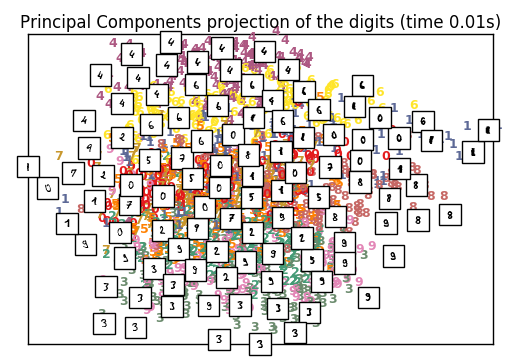
\includegraphics[scale=0.4]{tsne1.png}
	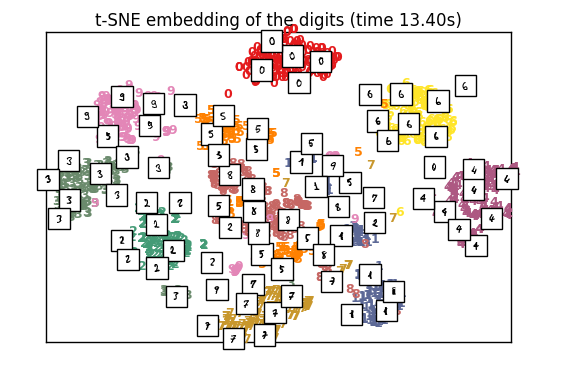
\includegraphics[scale=0.4]{tsne2.png}
\end{center}
Ici un exemple pour la classification de chiffres manuscrits. Les résultats sont bien meilleurs avec t-SNE mais hélas le temps de calcul est aussi bien plus long.